\documentclass{article}
\usepackage{tkz-graph} % from ctan or TL2011 one file tkz-graph.sty 

\begin{document}
  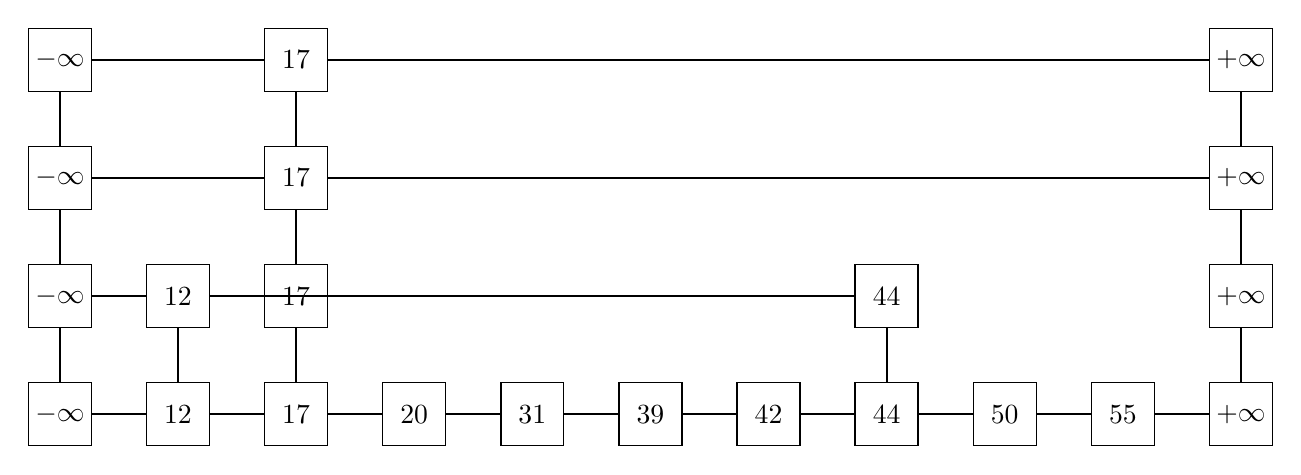
\begin{tikzpicture}
  \SetGraphUnit{1.5}
  \SetVertexNormal[Shape    = rectangle,MinSize=.8 cm]
   %%%%%%%%%%%%%%%%% vertices %%%%%%%%%%%%%%%%%%% 
   %  name of node x;y  x row y column

\Vertex[L=$-\infty$] {0;0}

\foreach \num [count=\n from 0] in  {1,2,3}
 {\NO[L=$-\infty$](0;\n){0;\num}}        
% No = north (initial node) {new node}  L=label 
\foreach \num/\label [count=\n from 0] in  
    {1/12,2/17,3/20,4/31,5/39,6/42,7/44,8/50,9/55,10/+\infty}
      {\EA[L=$\label$](\n;0){\num;0}} 
\foreach \num [count=\n from 0] in  {1,2,3}{%
     \NO[L=$+\infty$](10;\n){10;\num}}  

\foreach \num [count=\n from 0] in  {1,2,3} {%
    \NO[L=$17$](2;\n){2;\num}}   

\foreach \no/\label  in  {1/12,7/44} {%
    \NO[L=$\label$](\no;0){\no;1} } 

%%%%%%%%%%%%%%%%% edges %%%%%%%%%%%%%%%%%%%%%%%
 \foreach \num [count=\n from 1] in  {0,...,9}  {\Edge(\num;0)(\n;0)}

 \foreach \num [count=\n from 1] in  {0,...,2}  
 {\Edge(0;\num)(0;\n)  \Edge(2;\num)(2;\n)  \Edge(10;\num)(10;\n)}

\foreach \num  in  {1,7} {\Edge(\num;0)(\num;1)}   

\foreach \num [remember=\num as \lastnum (initially 0)] in  {2,10}  
 {\Edge(\lastnum;3)(\num;3) }  

\foreach \num [remember=\num as \lastnum (initially 0)] in  {2,10}  
 {\Edge(\lastnum;2)(\num;2)} 

\foreach \num [remember=\num as \lastnum (initially 0)] in  {1,7}  
 {\Edge(\lastnum;1)(\num;1)}     
   \end{tikzpicture}   
\end{document}